\chapter{Implementation} \label{implementation}

For this project I decided to use the Rust programming language. I chose
it because it makes performant, memory safe code much easier to write than
alternative systems languages such as C++ or C. Additionally, it has very good
parallel programming facilities and an extensive software ecosystem.

\subsection{Generating the Operator Precedence Table}

Setting up the precedence table for such grammars is a relatively
straightforward process. Initially, we determine the set FIRSTOP(A) for each
non-terminal A, representing the operators that can appear as the first operator
in sentential forms derived from A. It's important to note that this initial
operator can be preceded by at most one non-terminal in an operator grammar. The
construction of FIRSTOP sets for all non-terminals occurs simultaneously through
the following steps:

\begin{enumerate}

	\item For each non-terminal A, identify all right-hand sides of its rules.
	For each right-hand side R, include the first operator in R (if present) in
	FIRSTOP(A). This step establishes the initial values for all FIRSTOP sets.

    \item For each non-terminal A, examine all right-hand sides of its rules.
For each right-hand side R that commences with a non-terminal, denoted as
B, incorporate the elements of FIRSTOP(B) into FIRSTOP(A). This step is
justified by the possibility that a sentential form of A may initiate with B,
necessitating the inclusion of all operators in FIRSTOP(B) into FIRSTOP(A).

    \item Iteratively repeat step 2 until no further changes occur in any
FIRSTOP set. At this point, we have determined the FIRSTOP sets for all
non-terminals.
\end{enumerate}

Additionally, we require the set LASTOP(A), defined in a similar manner. An
analogous algorithm involves utilizing the last operator in R during step 1 and
incorporating the elements of FIRSTOP(B) where B terminates A in step 2. These
steps facilitate the determination of LASTOP sets.

\begin{listing}[H]
\begin{minted}[linenos]{text}
fn factorial[n: int] {
    if n == 0 {
        return 1;
    } 

    return (n * factorial(n - 1));
}
\end{minted}
\caption{Factorial in the test language.}
\label{lst:factorial_example}
\end{listing}

\begin{listing}[H]
\begin{minted}[linenos]{json}
{
  "a": 100,
  "b": {
    "x": [
      100,
      "a"
    ]
  }
}
\end{minted}
\caption{Example of parsable JSON.}
\hrulefill
\label{lst:json_example}
\end{listing}

Section \ref{dependancies}
\newline \newline
Section \ref{structure}
\newline \newline
Section \ref{outputs_and_visualizations}
\newline \newline
Section \ref{debugging}

\section{Dependencies} \label{dependancies}
\section{Structure} \label{structure}
\subsection{Parsing Grammar Transformation} \label{parsing_grammar_transformation}
\section{Outputs and Visualizations} \label{outputs_and_visualizations}

\begin{figure}[t]
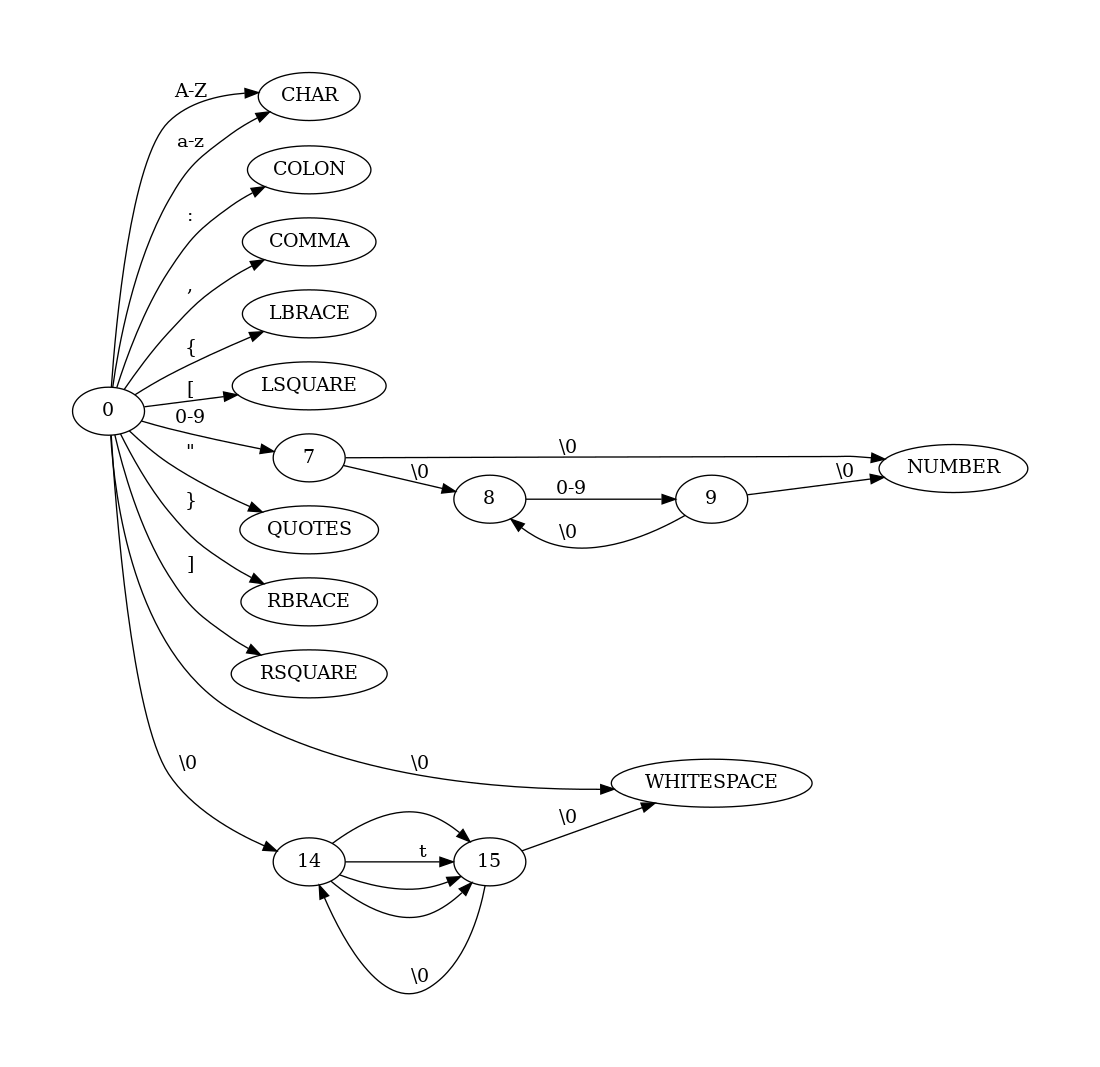
\includegraphics[width=\linewidth]{images/nfa.png}
\caption{NFA of the lexical grammar}
\label{fig:nfa}
\end{figure}

\begin{figure}[t]
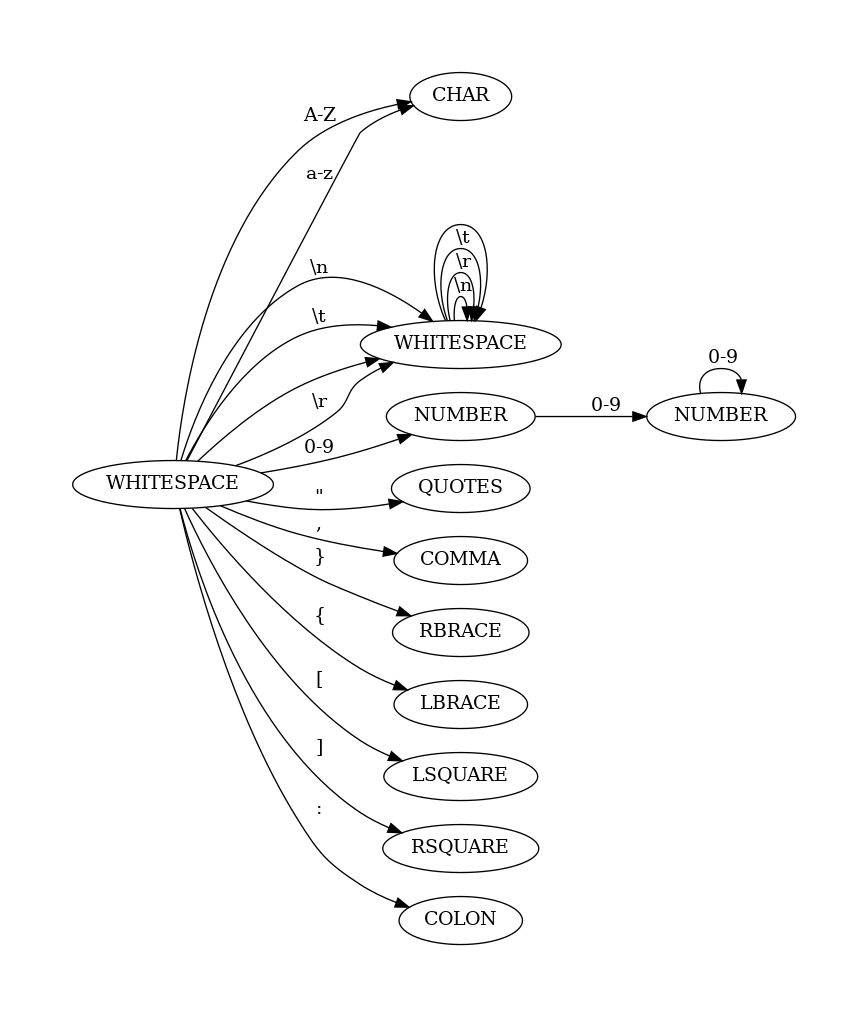
\includegraphics[width=\linewidth]{images/dfa.png}
\caption{DFA of the lexical grammar}
\label{fig:dfa}
\end{figure}

\begin{figure}[t]
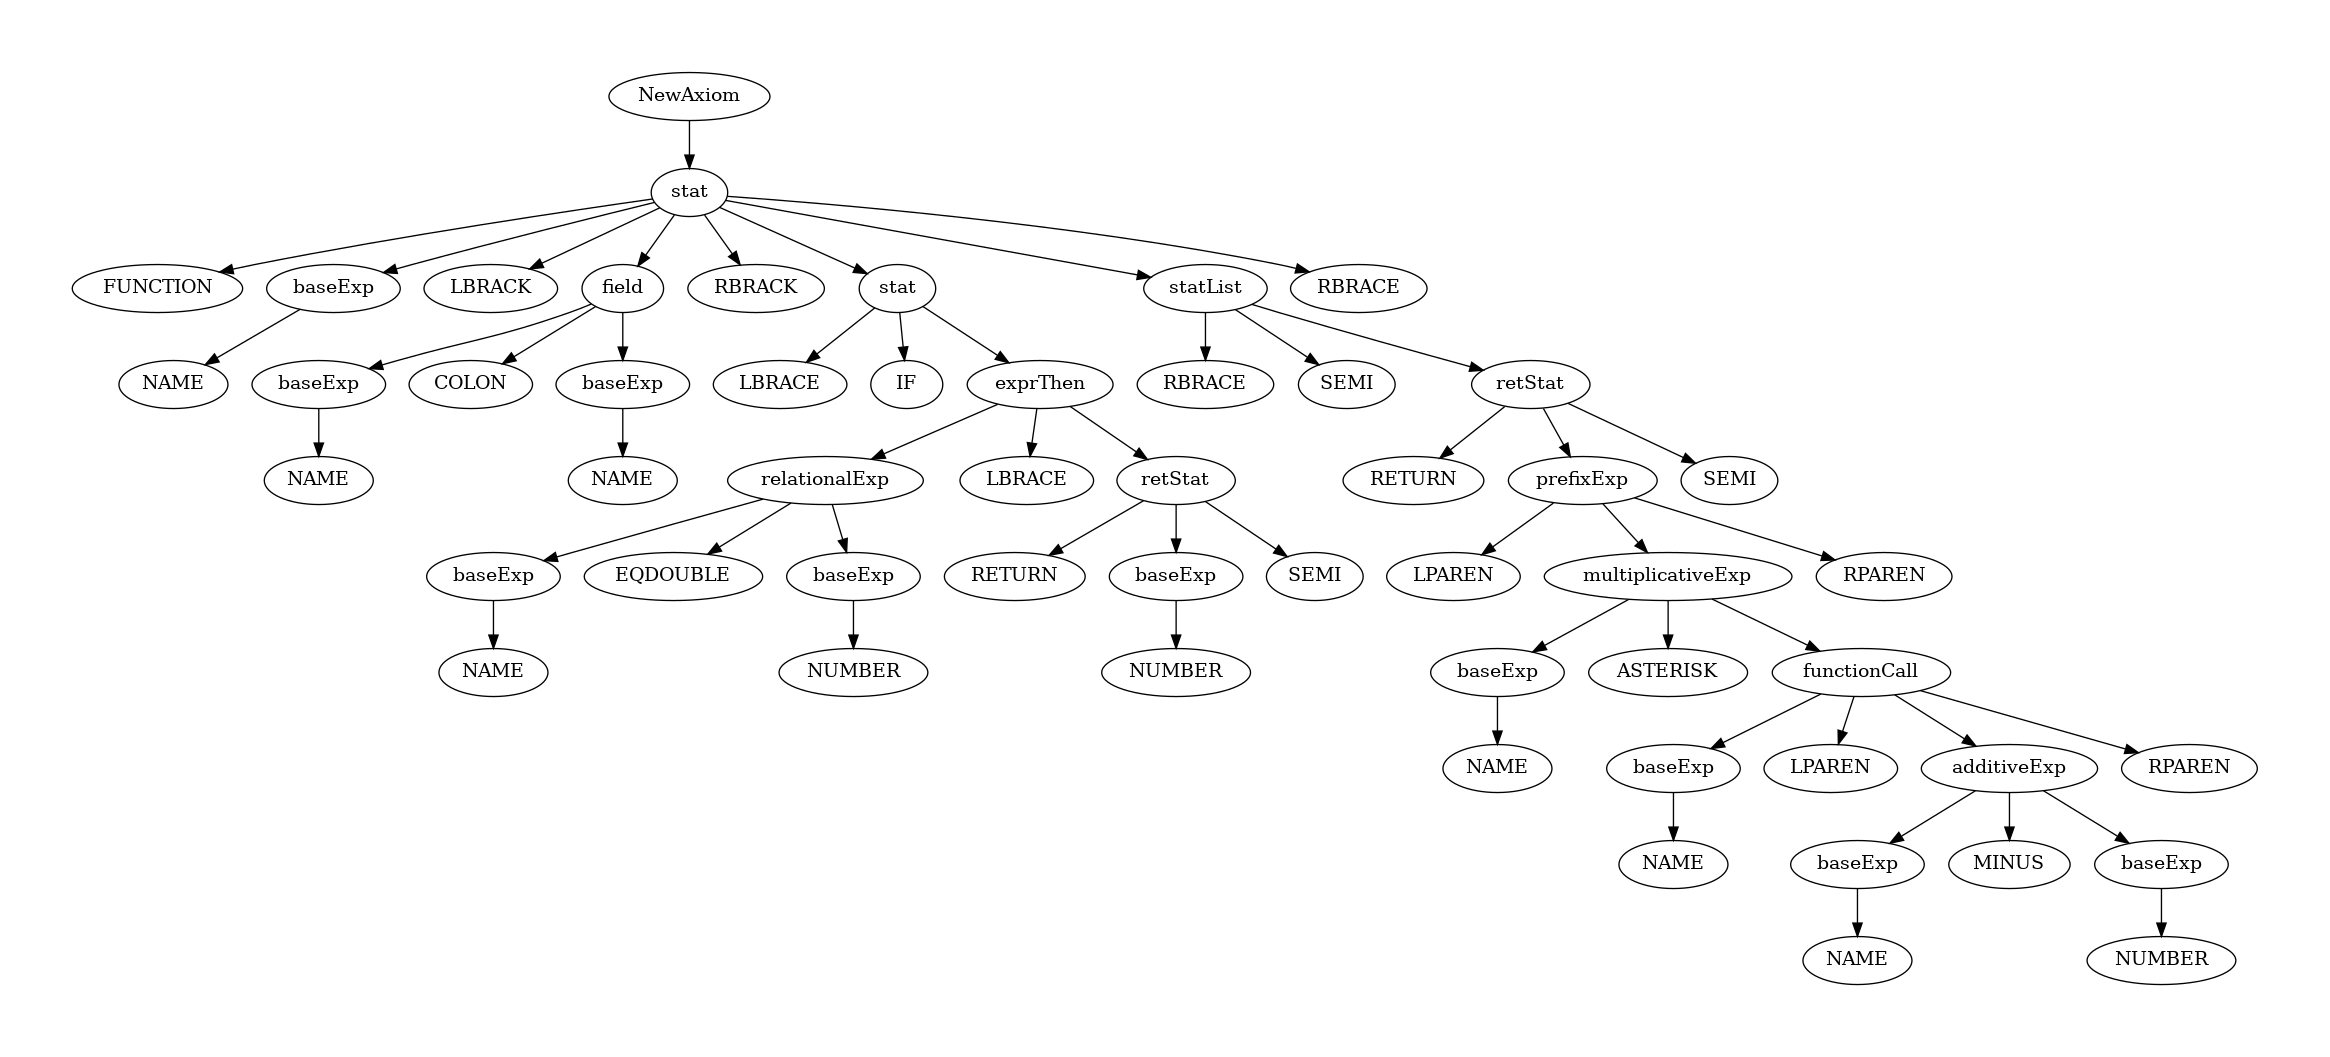
\includegraphics[width=\linewidth]{images/ptree.png}
\caption{Graphviz visualization of the parse tree.}
\label{fig:parse_tree}
\end{figure}

\section{Debugging} \label{debugging}
